\begin{figure}
\begin{tabular}{@{}c@{}c@{}}
\hspace{10px}
\begin{subfigure}[b]{0.48\textwidth}
\begin{center}
\begin{allLangEnvFoot}
~{\scriptsize \textcolor{mygray}{S0:}}~ List mk_list (i32 n) {
~{\scriptsize \textcolor{mygray}{S1:}}~   List l $\coloneqq$ LNil;
~{\scriptsize \textcolor{mygray}{S2:}}~   i32  i $\coloneqq$ ${\tt 0_{i32}}$;
~{\scriptsize \textcolor{mygray}{S3:}}~   while ${\tt \neg (i \geq_{u} n)}$:
~{\scriptsize \textcolor{mygray}{S4:}}~     l $\coloneqq$ LCons(i, l);
~{\scriptsize \textcolor{mygray}{S5:}}~     i $\coloneqq$ i + ${\tt 1_{i32}}$;
~{\scriptsize \textcolor{mygray}{S6:}}~   return l;
~{\scriptsize \textcolor{mygray}{SE:}}~ }
\end{allLangEnvFoot}
\vspace{40px}
\end{center}
\caption{\label{figr:llAllocSpecIR}(Abstracted) Spec IR}
\end{subfigure}%
&
\begin{subfigure}[b]{0.52\textwidth}
\begin{center}
\begin{allLangEnvFoot}
~{\scriptsize \textcolor{mygray}{C0:}}~ i32 mk_list (i32 n) {
~{\scriptsize \textcolor{mygray}{C1:}}~   i32 l $\coloneqq$ ${\tt 0_{i32}}$;
~{\scriptsize \textcolor{mygray}{C2:}}~   i32 i $\coloneqq$ ${\tt 0_{i32}}$;
~{\scriptsize \textcolor{mygray}{C3:}}~   while ${\tt i <_{u} n}$:
~{\scriptsize \textcolor{mygray}{C4:}}~     i32 p $\coloneqq$ malloc$_{\tt C4}$(sizeof(lnode));
~{\scriptsize \textcolor{mygray}{C5:}}~     $\mem{}$ $\coloneqq$ $\mem{}$[addrof($\structPointer{\tt p}{\mem{}}{lnode}{val}$)$\leftarrow$i]$_\type{i32}$;
~{\scriptsize \textcolor{mygray}{C6:}}~     $\mem{}$ $\coloneqq$ $\mem{}$[addrof($\structPointer{\tt p}{\mem{}}{lnode}{next}$)$\leftarrow$l]$_\type{i32}$;
~{\scriptsize \textcolor{mygray}{C7:}}~     l $\coloneqq$ p;
~{\scriptsize \textcolor{mygray}{C8:}}~     i $\coloneqq$ i + ${\tt 1_{i32}}$;
~{\scriptsize \textcolor{mygray}{C9:}}~   return l;
~{\scriptsize \textcolor{mygray}{CE:}}~ }
\end{allLangEnvFoot}
\end{center}
\caption{\label{figr:llAllocCIR}(Abstracted) C IR}
\end{subfigure}%
\\
\begin{subfigure}[b]{0.48\textwidth}
\begin{center}
{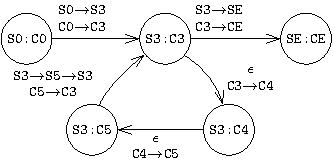
\includegraphics[scale=1.25]{chapters/figures/figMallocProductCfg.pdf}}
\end{center}
\caption{\label{figr:llAllocProductCFG}Product-CFG between IRs \\ in \cref{figr:llAllocSpecIR,figr:llAllocCIR}}
\end{subfigure}%
&
\begin{subfigure}[b]{0.52\textwidth}
\begin{center}
\begin{footnotesize}
% \begin{table}
\begin{tabular}{cll}
\toprule
{\bf PC-Pair} & \multicolumn{2}{c}{\bf Invariants} \\
\toprule
(\scpc{0}{0}) & \multicolumn{2}{l}{ $\circled{P}\  \sv{n} = \cv{n}$} \\
\midrule
\multirow{2}{*}{(\scpc{3}{3})} &  $\circled{\scriptsize I1}\  \sv{n} = \cv{n}$ & $\circled{\scriptsize I2}\  \sv{i} = \cv{i}$ \\
&  $\circled{\scriptsize I3}\  \sv{i} \leq_{u} \sv{n}$ & $\circled{\scriptsize I4}\  \sv{l} \indEq{} \lifted{list}{\mem{}}{lnode}{\cv{l}}$ \\
\midrule
(\scpc{3}{4}) &  $\circled{\scriptsize I5}\  \sv{n}=\cv{n}$ & $\circled{\scriptsize I6}\  \sv{i}=\cv{i}$ \\
(\scpc{3}{5}) &  $\circled{\scriptsize I7}\  \sv{i} <_{u} \sv{n}$ & $\circled{\scriptsize I8}\  \sv{l} \indEq{} \lifted{list}{\mem{}}{lnode}{\cv{l}}$ \\
\midrule
(\scpc{E}{E}) & \multicolumn{2}{l}{ $\circled{E}\  \sv{ret} \indEq{} \lifted{list}{\mem{}}{lnode}{\cv{ret}}$} \\
\bottomrule
\end{tabular}
% \end{table}
\end{footnotesize}
\end{center}
\caption{\label{tabr:llproductInv}Node invariants for product-CFG in \cref{figr:llAllocProductCFG}}
\end{subfigure}%
\\
\end{tabular}
\caption{\label{figr:llallocProductCFGAndInvs}\Cref{figr:llAllocSpecIR,figr:llAllocCIR} shows the IRs for the \SpecL{} and C {\tt mk\_list} procedures in \cref{fig:llAllocSpec,fig:llAllocC} respectively.
Product-CFG between the IRs in \cref{figr:llAllocSpecIR,figr:llAllocCIR} is shown in \cref{figr:llAllocProductCFG}.
\Cref{tabr:llproductInv} contains the corresponding node invariants for the product-CFG.}
\end{figure}